\documentclass[new]{subfiles}
\begin{document}

\newcommand{\ddP}[1]{\!\frac{\dd^3\vc#1}{(2\pi)^3}}

\section{Kinematics}
\subsection{Fundamentals}
$
\int\!\dd\Pi
= \int\ddP{p}\frac{1}{2E_{\vc p}}
= \int\!\frac{\dd^4 p}{(2\pi)^4}(2\pi)\ddelta\left((p^0)^2-m^2-\|\vc p\|^2\right)\Big|_{p^0\ge0}
$
\minisec{K\"all\'en function}
$
\mathop{\lambda}(x,y,z)
= x^2+y^2+z^2-2xy-2yz-2zx = (x-y-z)^2-4yz
$;\quad $\mathop{\lambda}(s,m_1^2,m_2^2)=s^2\mathop{\lambda}(1,m_1^2/s,m_2^2/s)$;\\
$
\mathop{\lambda}(1;\alpha_1^2,\alpha_2^2)
= (1-(\alpha_1+\alpha_2)^2)(1-(\alpha_1-\alpha_2)^2)
= (1+\alpha_1+\alpha_2)(1-\alpha_1-\alpha_2)(1+\alpha_1-\alpha_2)(1-\alpha_1+\alpha_2).
$
\begin{align}
\mathop{\lambda^{1/2}}\left(1;\frac{m_1^2}{s},\frac{m_2^2}{s}\right)
= \sqrt{1-\frac{2 (m_1^2+m_2^2)}{s}+\frac{(m_1^2-m_2^2)^2}{s^2}};\quad
m_1=m_2:\ \sqrt{1-\frac{4m^2}{s}},\quad
m_2=0:\ \frac{s-m_1^2}{s}.
\end{align}


\paragraph{Two-body kinematics}
$s=(p_1+p_2)^2$\\
In CM frame, $s=(E_1+E_2)^2$ and
$p= \sqrt{\frac{s}{4}}\mathop{\lambda^{1/2}}\left(1;\frac{m_1^2}{s},\frac{m_2^2}{s}\right)$;
\quad
$E_1 = \frac{s+m_1^2-m_2^2}{2\sqrt{s}}$.
\\
For $m_1=m_2$, $E=\frac{\sqrt{s}}{2}$ and $
p = \sqrt{\frac{s}{4}}\sqrt{1-\frac{4 m^2}{s}}
=\frac{\sqrt{s-4m^2}}{2}$; $v=\frac{p}{E}=\sqrt{1-\frac{4m^2}{s}}$.
\\
For $m_2=0$, $p=\frac{\sqrt{s}}{2}\left(1-\frac{m_1^2}{s}\right)=E_2$ and
$E_1=\frac{\sqrt{s}}{2}\left(1+\frac{m_1^2}{s}\right)$.
\minisec{Two-body phase space}
$
\int\!\dd\Pi_1\dd\Pi_2\text{(Lorentz invariant)}
= \int\!\dd\Pi_1\dd\Pi_2\,f(p_1, p_2, p_1^\mu p_{2\mu})
= \int\!\dd\Pi_1\dd\Pi_2\,f(p_1,p_2,\cos\theta_{12}).
$
\\
Rewriting with $E_\pm = E_1\pm E_2$ and $s=(p_1+p_2)^2=m_1^2 + m_2^2 + 2E_1E_2 - \|\vc p_1\|\|\vc p_2\|\cos\theta_{12}$,
\\
$
\int\dd\Pi_1\dd\Pi_2
=
\int\ddP{p_1}\,\,\ddP{p_2}\frac{1}{2E_12E_2}
=
\int\!\frac{(4\pi)\dd p_1\,p_1^2}{(2\pi)^3}
\frac{(2\pi)\dd p_2\,p_2^2\,\dd\cos\theta_{12}}{(2\pi)^3}\frac{1}{2E_12E_2}
=
\int\!\frac{\dd E_+\dd E_- \dd s}{32\pi^4}
$,
\\
where the Jacobian is $\left|\frac{\dd(E_+,E_-,s)}{\dd(p_1, p_2, \cos\theta_{12})}\right|=\frac{4p_1^2p_2^2}{E_1E_2}$, or $\left|\frac{\dd(E_1,E_2,s)}{\dd(p_1, p_2, \cos\theta_{12})}\right|=\frac{2p_1^2p_2^2}{E_1E_2}.$
\\
As $
\cos\theta_{12}=\frac{E_+^2-E_-^2+2 \left(m_1^2+m_2^2-s\right)}{\sqrt{(E_++E_-)^2-4 m_1^2}\sqrt{(E_+-E_-)^2-4 m_2^2}}
$ is restricted as $[-1,1]$, $E_-$ is bounded as
\\
$
\left|E_- - \frac{m_1^2-m_2^2}{s}E_+\right| 
\le
\sqrt{E_+^2-s}\cdot\mathop{\lambda^{1/2}}\left(1;\frac{m_1^2}{s},\frac{m_2^2}{s}\right)
=
2p\sqrt{\frac{E_+^2-s}{s}}
$; using these bounds,
\begin{equation}
 \int\dd\Pi_1\dd\Pi_2
=
\frac{1}{32\pi^4}
\int_{(m_1+m_2)^2}^\infty\dd s
\int_{\sqrt{s}}^\infty\dd E_+
\int\w{min}^{\mathrm{max}}\dd E_-.
\end{equation}

\minisec{Two-body phase space with momentum conservation}
$\int\dd\Pi^{(2)}:=
\int\dd\Pi_1\dd\Pi_2\,(2\pi)^4\ddelta[4](P_0-p_1-p_2)
=
\int\!\frac{\dd p_1\dd\Omega\,p_1^2}{16\pi^2}\frac{\delta(E_0-\sqrt{m_1^2+p_1^2}-\sqrt{m_2^2+\|\vc P_0-\vc p_1\|^2})}{E_1E_2}
$;
\\
$p_1=\frac{(E_0^2+m_1^2-m_2^2-P_0^2)P_0\cos\theta_1
 + E_0\sqrt{\mathop{\lambda}(E_0^2,m_1^2,m_2^2)+P_0^4-2P_0^2(E_0^2+m_1^2-2m_1^2\cos^2\theta_1-m_2^2)}
}{2(E_0^2-P_0^2\cos^2\theta_1)}$\\
and
$
\int\dd\Pi^{(2)}
=
\frac{1}{8\pi}\int\dd\cos\theta_{1}\frac{p_1^2}{E_0p_1-P_0E_1\cos\theta_1}
$;
\begin{align}
 \text{CM ($E_0=\sqrt{s}$):}& &
\int\dd\Pi^{(2)}&=\int\frac{\dd\cos\theta_{1}}{8\pi}\frac{p}{\sqrt{s}}
;&
 p &= \frac{\sqrt{s}}{2}\mathop{\lambda^{1/2}}\left(1;\frac{m_1^2}{s},\frac{m_2^2}{s}\right),
&
E_1 &= \frac{s+m_1^2-m_2^2}{2\sqrt{s}}.
\end{align}

\newpage
\subsection{Decay rate and Cross section}
\noindent
Rate $\dd R=\dd\Pi^{(n)}\left|\mathcal M\right|^2(2\pi)^4\ddelta[4](p\w i-p\w f)$ is Lorentz invariant; density is given by $\rho=2E$.
\\
Decay rate: $R = \frac{N}{VT} =: \rho_1^{\text{rest}}\Gamma = 2m\Gamma$\quad(defined at the rest frame);
\\
Cross section:
$R = \frac{N}{VT}
=: v\w{rel}\rho_1\rho_2 \frac{p_1\cdot p_2}{E_1E_2}\sigma=:v_{\text{M\o l}}\rho_1\rho_2\sigma$\quad (defined as Lorentz invariant).
\\
Note that $\rho/E$ is Lorentz invariant; the factor is introduced as $(p_1\cdot p_2)/E_1E_2=1$ at $\vc p_1=0$ or $\vc p_2=0$.
\begin{align}
&\text{relative velocity:}\quad
v\w{rel}
=
\frac{\sqrt{(p_1\cdot p_2)^2-m_1^2m_2^2}}{p_1\cdot p_2}
=
\frac{\sqrt{\|\vc v_1-\vc v_2\|^2-\|\vc v_1\times\vc v_2\|^2}}{1-\vc v_1\cdot\vc v_2}
=
\frac{\mathop{\lambda^{1/2}}(s,m_1^2,m_2^2)}{s-(m_1^2+m_2^2)},
\\
&\text{M\o ller parameter:}\quad
v_{\text{M\o l}}:= \frac{\sqrt{(p_1\cdot p_2)^2-m_1^2m_2^2}}{E_1E_2}\quad \leadsto \text{$|v_1-v_2|$ if $\vc v_1\parallel \vc v_2$};
\end{align}
\vspace{-1em}\par
{\hfill [mass dimension of $\mathcal M$ is $4-N\w i-N\w f$]}
\par\vspace{-2.4em}
\begin{align}
\dd\Gamma&=
\frac{1}{2m_A}\Biggl[\prod\w f\frac{\dd^3p\w f}{(2\pi)^3}\frac{1}{2E\w f}\Biggr]
\Bigl|\mathcal M(m_A\to\{p\w f\})\Bigr|^2(2\pi)^4\ddelta[4]\left(m_A-\{p\w f\}\right),
\\
\dd\sigma &=
\frac{1}{2E_A2E_B\ v_{\text{M\o l}}}\Biggl[\prod\w f\frac{\dd^3p\w f}{(2\pi)^3}\frac{1}{2E\w f}\Biggr]
\Bigl|\mathcal M(p_A,p_B\to\{p\w f\})\Bigr|^2(2\pi)^4\ddelta[4]\left(p_A+p_B-\{p\w f\}\right).
\end{align}

\minisec{Two-body kinematics in CM frame}
\begin{align}
\int\!\dd\Pi^{(2)}
&:=\int\!\frac{\dd^3\vc p_1}{(2\pi)^3}\frac{\dd^3\vc p_2}{(2\pi)^3}
\frac{1}{2E_1}\frac{1}{2E_2}\,(2\pi)^4\ddelta[4](\sqrt{s}-p_1-p_2)\qquad\text{($\sqrt s=E\w{CM}$ or $M\w{mother}$)}
\notag\\&=
\frac{\|\vc p\|}{4\pi\sqrt{s}}\int\!\frac{\dd\Omega}{4\pi}
=
\frac{\|\vc p\|}{8\pi \sqrt{s}}\int\dd\cos\theta
\\
\frac{\|\vc p\|}{8\pi\sqrt{s}}
&=
\frac{1}{8\pi\sqrt{s}}\cdot\frac{\sqrt{s}}{2}\mathop{\lambda^{1/2}}\left(1;\frac{m_1^2}{s},\frac{m_2^2}{s}\right)
=
\frac1{16\pi}\sqrt{1-\frac{2 (m_1^2+m_2^2)}{s}+\frac{(m_1^2-m_2^2)^2}{s^2}}
\end{align}
\begin{align}
 E_1&=\frac{s+m_1^2-m_2^2}{2\sqrt{s}}&
 E_2&=\frac{s-m_1^2+m_2^2}{2\sqrt{s}}&
 p_1\cdot p_2 &= \frac{s-(m_1^2+m_2^2)}{2}
\end{align}

\subparagraph{Mandelstam variables} For $(k_1,k_2)\to(p_3,p_4)$ collision,
\begin{align*}
 &s = (k_1+k_2)^2 = (p_3+p_4)^2, \quad
 t = (p_3-k_1)^2 = (p_4-k_2)^2, \quad
 u = (p_3-k_2)^2 = (p_4-k_1)^2;\\
 & s+t+u=m_1^2+m_2^2+m_3^2+m_4^2
\end{align*}

\begin{wrapfigure}[3]{r}{10.1em}
\vspace{-2em}
 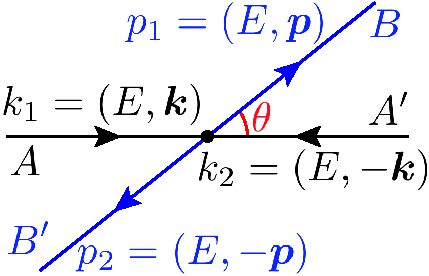
\includegraphics[width=10em]{collision.pdf}
\end{wrapfigure}
For same-mass collision, $ s = (2E)^2 = E\w{CM}^2$ and
\begin{align*}
 t &= m_A^2+m_B^2 - s/2+2kp\cos\theta
&
(k_1-k_2)^2&=4m_A^2-s
\\
 u &= m_A^2+m_B^2 - s/2-2kp\cos\theta
&
(p_1-p_2)^2&=4m_B^2-s
\end{align*}\vspace{-1.5em}
\begin{align*}
 k&=\frac{\sqrt{s-4m_A^2}}{2}
&k_1\cdot k_2 &= \frac{s}{2}-m_A^2
&k_1\cdot p_1&=k_2\cdot p_2=\frac{m_A^2+m_B^2-t}{2}
\\
 p&=\frac{\sqrt{s-4m_B^2}}{2}
&p_1\cdot p_2 &= \frac{s}{2}-m_B^2
&k_1\cdot p_2&=k_1\cdot p_2=\frac{m_A^2+m_B^2-u}{2}
\end{align*}
\begin{wrapfigure}[3]{r}{10.1em}
\vspace{-1.5em}
 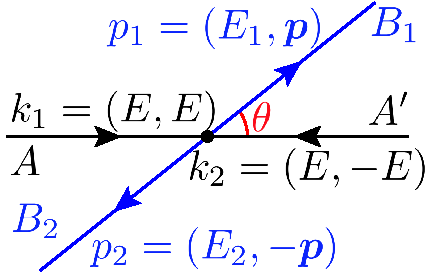
\includegraphics[width=10em]{collision2.pdf}
\end{wrapfigure}

For collision with initial mass ignored,
\begin{align*}
 t &= (m_1^2+m_2^2-s)/2+p\sqrt{s}\cos\theta\\
 u &= (m_1^2+m_2^2-s)/2-p\sqrt{s}\cos\theta
\end{align*}



\end{document}
